\Chapter{Tesztelés}

\Section{Felhasználói kézikönyv}
\label{sec:installation}

Ahhoz, hogy az AI ellen tudjunk játszani, először telepítenünk kell az OpenTTD-t. Ha ez megtörtént, a DebacleAI fájljait a játék mappájában lévő \texttt{ai} nevű mappába kell bemásolnunk. Ennek az útvonala alapértelmezett telepítési beállítások mellett Windows-on "\texttt{C:\textbackslash Program Files\textbackslash OpenTTD\textbackslash ai}". Miután bemásoltuk a DebacleAI mappáját a játékéba, az elindítást követően az "MI/Játékszkript beállítások" menüpontban van lehetőség gépi ellenfél hozzáadására. Az ilyenkor megnyíló helyre be lehet állítani a DebacleAI-t, mint ellenfél. Ezt követően egy új játék megkezdésekor az AI automatikusan el fog indulni.

Ezek után egyéb figyelmet az AI nem igényel, a felhasználó szabadon játszhat a játékkal, miközben az AI is a korábban bemutatott módon fogja játszani a játékot, mint egy rivális cég a pályánkon.

Abban az esetben, ha az AI futás idejű problémába ütközne, a játék értesíteni fogja erről a felhasználót. Ebben az esetben a nyomkövetés ablakában lévő MI újratöltése gombbal van lehetőségünk újraindítani az AI-t. Ennek az ablaknak magától is meg kellene nyílnia, de abban az esetben, ha ez nem történne meg, a felső eszközsáv utolsó gombját (kérdőjel egy kék körben) lenyomva tartja tudjuk elérni az "MI/Játékszkript nyomkövetés" pontban.

\Section{Megfigyelések}

Már a rövid fejlesztési folyamat közben is észrevehető volt, hogy az AI képes a játékmenet fenntartására, és nyereség generálására is, tehát ebből a szempontból a saját stratégia megvalósítása sikeresnek nevezhető. Ugyanakkor, a DebacleAI csak utasok szállításával foglalkozik buszok segítségével, a többi szállítási lehetőség egyáltalán nincs lefedve az AI által.

Ezzel szemben más AI-oknak sokkal fejlettebbek. Az általános AI-ok minden szállítási lehetőséggel, és sokkal stabilabban futnak, kevesebb hibába ütköznek, és több profitot is képesek generálni. Ez annak is betudható, hogy a legtöbb AI éveken keresztül haladt át a fejlesztési folyamaton és ennél még hosszabb tesztelési fázison. Közben és után, elérhető volt a játékosbázis részére, így játékosok százai tudták kipróbálni őket, és visszajelzést adni adott hibákról, problémákról vagy ötletekkel hozzájárulni a folyamathoz. A fórumbejegyzéseket olvasva megállapítható, hogy a problémák többsége ami felléphet a játék folyamán a következők.
\begin{itemize}
	\item Útvonal/hálózat tervezéssel kapcsolatos problémák.
	\item Útvonalkereső hatékonyságához köthető hibák.
	\item Adott út/vasúthálózatok túlterhelése járművekkel.
	\item Pénzügyi problémákkal kapcsolatos észrevételek.
	\item Létező infrastruktúra újrahasznosításával kapcsolatos problémák.
\end{itemize}
Ebből a lényeges információ amire következtethetünk, hogy függetlenül az AI fejlesztési idejétől vagy a tesztelők számától, még a legrégebbi és legátfogóbb AI-okban is jelentkezhetnek problémák. Ezeket a megszokott módon a fórumbejegyzésekben szokták megtenni. Megfigyelhető, hogy 10 évvel ezelőtt fejlesztett AI-ok bejegyzéseiben még a tavalyi év folyamán is érkeztek bejelentések hibákról. Tekintve, hogy a játék környezete nagyon dinamikus, és az AI megvalósításának problémája mennyire komplex, nehéz teljesen ideális, vagy hibátlan állapotot elérni.

Ahogyan \aref{fig:atlag}. ábrán megfigyelhető, egy átlagos futtatási szituációban az AI jó eredményeket képes produkálni. Itt látható, hogy a 10 éves folyamat alatt:
\begin{itemize}
	\item 152 jármű zárta profittal az előző évet,
	\item A közelmúltban 67 állomást szolgált ki,
	\item Az előző negyedév profitja 74 százalékkal nagyobb az elmúlt 12 negyedév maximális profitjánál,
	\item 22.147 utast szállítottunk el ez előző negyedévben,
	\item Az felvett kölcsön mennyisége 0.
\end{itemize}

\begin{figure}
	\centering
	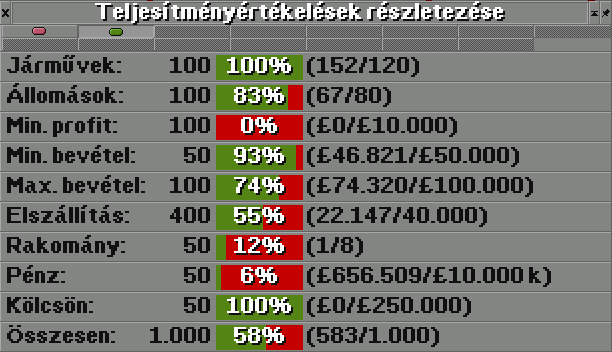
\includegraphics[width=\textwidth]{images/atlag.png}
	\caption{A DebacleAI kiértékelése egy 10 éves játékfolyamat után.}
	\label{fig:atlag}
\end{figure}

\Section{Tesztelési körülmények}

A következő részekben az AI-ok teljesítményének az összehasonlítását fogom bemutatni. Ehhez az AI-okat egy játékkörnyezetben futtattam 10 évig. Ezekben a játékokban, a pályagenerálás beállításai mindig ugyan azok voltak. Ezek pedig az alábbiak.
\begin{itemize}
	\item Térkép mérete: $256 \times 256$
	\item Térkép generátor: TerraGenesis
	\item Várossűrűség: Normál
	\item Gazdasági épületek száma: Normál
	\item Tereptípus: Sík
	\item Tengerszint: Nagyon alacsony
	\item Simaság: Sima
	\item Folyók: Közepes
	\item Dátum: 1950 Január 1.
	\item A térkép határa minden esetben víz
\end{itemize}

Az olyan AI-ok esetében, ahol a megvalósítás általános, és többféle szállítási módszert is tudnak használni, a működést lekorlátoztam buszok használatára. (A SimpleAI esetében erre nem volt lehetőség, azt csak közúti járművekre lehet korlátozni.) Ennek az volt az oka, hogy összehasonlítás szempontjából, az olyan AI-okkal szemben amelyek csak utasokat szállítanak, vagy csak közúti járműveket használnak, sokkal nagyobb bevétel generálására lettek volna képesek a piaci rés kihasználásával.

\Section{Önálló tesztelés}

A korábban felsorolt tesztkörülmények között tesztelve a DebacleAI-t csak önmagában, rivális cégek nélkül \aref{tab:debacle20}. táblázatban látható eredményeket volt képes produkálni egy 20 éves tesztfuttatás alatt.

Ez a teszt megerősítette a korábban mért teljesítményét az AI-nak, ugyanis hasonló teljesítménnyel rendelkezik a tesztkörülmények alatt is, mint amivel a fejlesztés folyamata alatt rendelkezett.

\begin{table}
	\centering
	\caption{DebacleAI futtatásának eredményei 20 éven keresztül a tesztkörülmények között}
	\label{tab:debacle20} 
	\smallskip
	\begin{tabular}{|l || c | c | c | c |} 
		\hline
		\texttt{Év} & 1955 & 1960 & 1965 & 1970 \\ 
		\hline\hline
		Cég kora & 5 év & 10 év & 15 év & 20 év  \\ 
		\hline
		Cég értéke &  \pounds 351.896 & \pounds 520.168  & \pounds 1.073.358 & \pounds 2.271.429\\
		\hline
		Járművek előző évi bevétele & +\pounds 177.296 & +\pounds 227.190  & +\pounds 367.574 & +\pounds 707.739 \\
		\hline
		Járművek száma (nyereséges) & 62/95 & 99/149 & 126/188 & 208/298 \\
		\hline
		Állomások száma & 38 & 58 & 62 & 108 \\ 
		\hline
		Elszállított utasok száma & 8.818 & 11.816 & 18.740 & 35.416  \\
		\hline
		Teljesítmény értékelés & 235 & 314 & 476 & 760 \\ 
		\hline
	\end{tabular}
\end{table}

\Section{Rivális céggel való összevetés}

Ebben a szakaszban az AdmiralAI-t választottam, mint rivális cég. Ennek az oka az volt, hogy az AdmiralAI az egyik leggyakoribban használt AI a játékon belül, valamint annak ellenére, hogy az AI megvalósítása általános, a beállításai módosításával elérhető, hogy csak buszokat használjon. Ennek az összevetésnek az eredményei \aref{tab:debvsadm}. táblázatban láthatóak.

Ahogyan a táblázatból is leolvasható, a DebacleAI nyereségben, és ősszesített pontok alapján is az AdmiralAI mögött helyezkedik el. Azonban ez korántsem meglepő megállapítás. A két AI fejlesztési idejének különbségéhez képest, a teljesítménybeli eltérések egészen alacsonyak. A tesztfolyamat közben észrevehető volt, hogy a DebacleAI pár év lemaradással, ugyan azt a tendenciát követte a bevétel szempontjából, mint az AdmiralAI. A DebacleAI a város és buszmegálló keresése közben, mindig az ideálisat igyekszik megtalálni, és próbálja minimalizálni a rivális cégekkel való osztozkodást az utasokon. Emiatt többször is előfordult a játék állapotát figyelve, hogy az AdmiralAI terjeszkedése gyorsabb volt, így kizárta egy adott városba való terjeszkedését a DebacleAI-nak. Az tesztfolyamat utolsó 6 évében a vállalat értékének alakulását \aref{fig:dvafug}. ábrán láthatjuk.

\begin{figure}
	\centering
	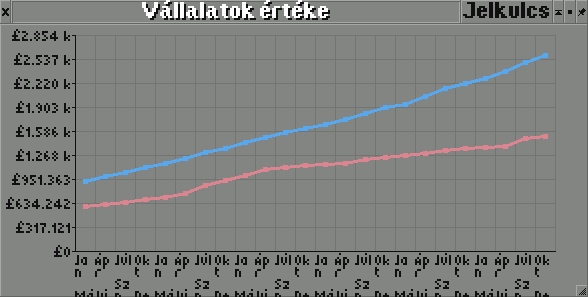
\includegraphics[width=\textwidth]{images/valert.png}
	\caption{A DebacleAI(Rózsaszín) és AdmiralAI(Kék) Cég értékét ábrázoló grafikon az utolsó 20 negyedévre nézve.}
	\label{fig:dvafug}
\end{figure}

\begin{landscape}
\begin{table}
	\centering
	\caption{DebacleAI és AdmiralAI teljesítménye 15 éves tesztfuttatás alatt.}
	\label{tab:debvsadm}
	\smallskip
	\begin{tabular}{|c || c | c | c | c | c | c |} 
		\hline
		AI: & \texttt{DebacleAI} & \texttt{AdmiralAI} & \texttt{DebacleAI} & \texttt{AdmiralAI} & \texttt{DebacleAI} & \texttt{AdmiralAI} \\
		\hline
		\texttt{Év:} & \multicolumn{2}{c|}{1955} & \multicolumn{2}{c|}{1960} & \multicolumn{2}{c|}{1965} \\
		\hline\hline
		\hline
		Cég kora: & \multicolumn{2}{c|}{5 év} & \multicolumn{2}{c|}{10 év} & \multicolumn{2}{c|}{15 év} \\ 
		\hline
		Cég értéke: &  \pounds 187.568 & \pounds 375163  & \pounds 681.090 & \pounds 1.090.532 & \pounds 1.586.468 & \pounds 2.537.945 \\
		\hline
		Közúti járművek bevétele(előző év) & +\pounds 142.086 & +\pounds 174.440  & +\pounds 284.796 & +\pounds 376.991 & +\pounds 480.880 & +\pounds 817.567 \\
		\hline
		Járművek száma(ebből nyereséges) & 51/76 & 85/96 & 121/154 & 174/217 & 200/298 & 376/440 \\
		\hline
		Állomások száma & 26 & 18 & 48 & 44 & 92 & 71 \\ 
		\hline
		Elszállított utasok száma: & 7.673 & 8.477 & 13.168 & 14.194 & 23.114 & 27.620  \\
		\hline
		Teljesítmény értékelés: & 192 & 237 & 374 & 417 & 549 & 618 \\ 
		\hline
	\end{tabular}
\end{table}
\end{landscape}

\Section{Városkereső algoritmus hangolása}

Az előző fejezetben bemutatott városkereső algoritmus rendelkezik egy súly paraméterrel. Ennek az állításával tudjuk meghatározni, hogy a városok távolságát, vagy a rendelkezésre álló utasok számát szeretnénk-e inkább figyelembe venni.  Ezt a paramétert a $[0, 1]$ intervallum között tudjuk állítani. A tesztesetek pedig a $[0.1, 0.9]$ intervallumon végeztem el $0.1$-es lépésközzel. Ezeknek a mérésnek az adait \aref{fig:meresek}. ábrán lehet látni. A cég bevételén kívül megvizsgáltam még a megépített utak és a buszmegállók számát is, ezek \aref{fig:utak}. és \aref{fig:wmegallok}. ábrákon láthatóak.

\begin{figure}
	\centering
	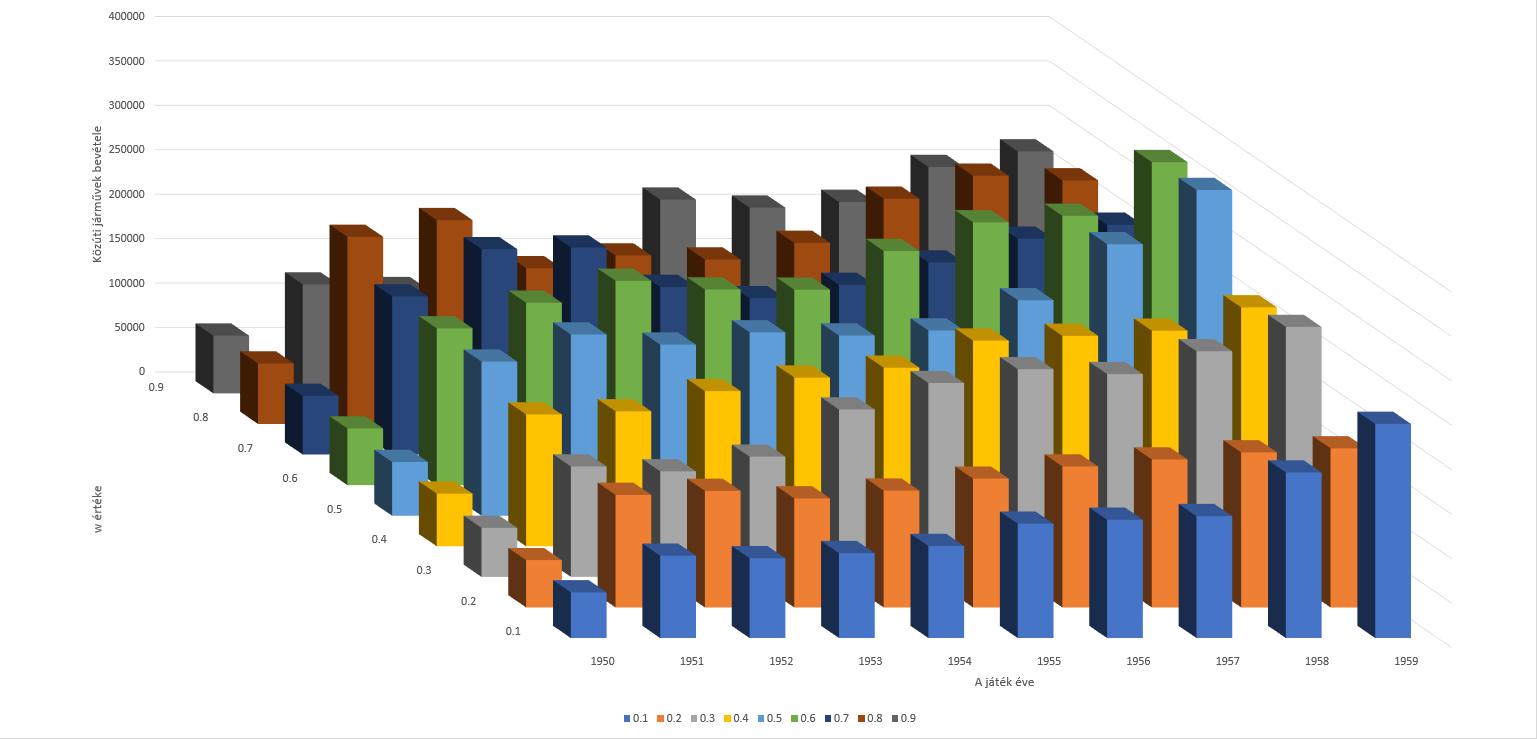
\includegraphics[width=\textwidth]{images/wmeresek.png}
	\caption{A DebacleAI bevételének változása a $w$ értékétől függően.}
	\label{fig:meresek}
\end{figure}

\begin{figure}
	\centering
	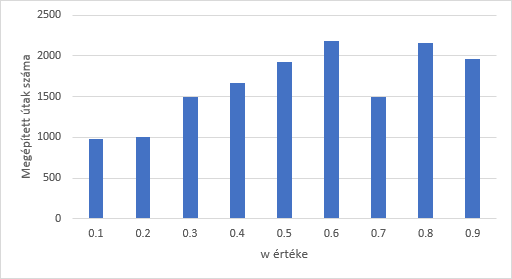
\includegraphics[width=\textwidth]{images/wutak.png}
	\caption{A DebacleAI által épített utak mennyiségének változása a $w$ értékétől függően.}
	\label{fig:utak}
\end{figure}

\begin{figure}
	\centering
	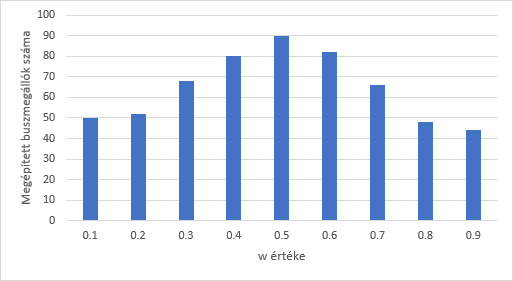
\includegraphics[width=\textwidth]{images/wallomas.png}
	\caption{A DebacleAI által épített buszmegállók mennyiségének változása a $w$ értékétől függően.}
	\label{fig:wmegallok}
\end{figure}

A tesztelés folyamán nyert tapasztalatok a következőkben foglalhatók össze.
\begin{itemize}
	\item Az első év eredményei nagyon hasonlítanak egymásra, mivel itt az AI minden beállítás mellett felveszi a maximális kölcsön mennyiségét, és annyi útvonalat épít ki belőle amennyi lehetséges, így az egy éven belül megépített útvonalak megegyeznek a kölcsön miatt, a második évre, ezeknek a profitja miatt már észlelhetőek eltérések a bevételben.
	\item Minél kisebb a $w$ értéke, annál kevesebb utat épít az AI, mivel a távolságot jobban figyelembe veszi, mint az utasok számát. A $[0.5, 0.6]$ tartományon csúcsosodik, aztán tovább növelve a $w$-t ismét csökkenni kezd az utak száma. Ez amiatt van, mivel a magas $w$ értékeknél, az algoritmus nem figyelte annyira az adott városok távolságát, emiatt messzebb lévő városokat is megpróbált összekötni. Azonban az útvonalkereső nem tudta a lépést tartani ezzel, és egyes útvonalak kiépítése hónapokba telt. Feltételezem, hogy ha gyorsabban meg tudta volna keresni az útvonalat az algoritmus, a megépített utak száma a nagyobb $w$ értékeknél továbbra is egyre nagyobb lett volna.
	\item Az előző pontban említett messzi városok összekötése miatt történt az is, hogy a magasabb $w$ értékeknél kevesebb megálló került építésre, azaz kevesebb útvonal lett létrehozva.
	\item Az évek haladtával észrevehető, hogy azonos $w$ értéknél egymást követő éveken keresztül ugyan akkora a bevétel. Ezt a tesztelés közben a nyomkövető ablakot vizsgálva annak tudható be, hogy amikor a cég eléri a maximális kölcsön méretet és várnia kell, amíg elegendő pénzmennyiség összegyűlik egy új vonal megépítéséhez, miközben a buszokat is kezeli.
	\item A nagyobb $w$ értékek esetében az első években a cég bevétele nagyobb, azonban a későbbiekben lemarad az alacsonyabbakéhoz képest.
	\item A tesztelés során a legmagasabb bevételi értéket, ami \pounds 366480 volt, a 0.5-ös $w$ értékkel érte el a program. A megépített buszmegállók számából megfigyelhető még, hogy a 0.5-ös értéknél lett létrehozva a legtöbb vonal is a pályán. Ez ebben az esetben a megépített megállók fele, azaz 45.
\end{itemize}
